% Source: http://tex.stackexchange.com/a/69234/5645
\documentclass[varwidth=true, border=2pt]{standalone}

\usepackage{pgfplots}

\begin{document}
    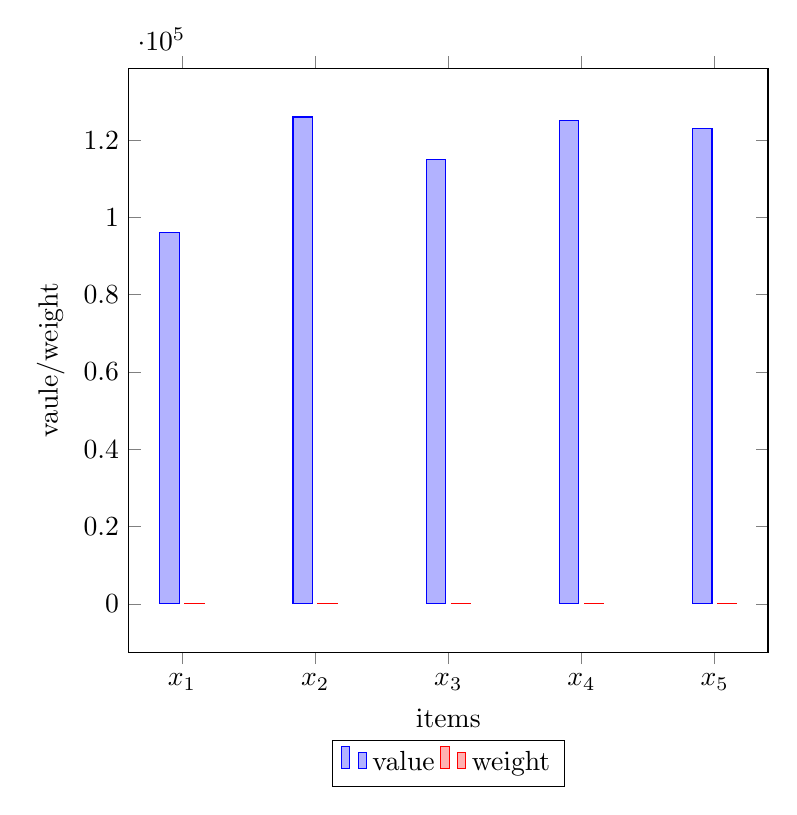
\begin{tikzpicture}
        \begin{axis}[
            ybar,
            ylabel={vaule/weight},
            xlabel={items},
            legend style={at={(0.5,-0.15)},
            anchor=north,legend columns=-1},
            width=0.8*\textwidth,
            height=9cm,
            bar width=7pt,
            symbolic x coords={$x_1$,$x_2$,$x_3$,$x_4$,$x_5$},
            xtick=data,
            %nodes near coords,
            %nodes near coords align={vertical},
        ]
            \addplot
            coordinates {($x_1$,96000) ($x_2$,126000) ($x_3$,115000) ($x_4$,125000) ($x_5$,123000)};
            \addplot
            coordinates {($x_1$,27) ($x_2$,21) ($x_3$,27)  ($x_4$,15) ($x_5$,19)};
            \legend{value, weight}
        \end{axis}
    \end{tikzpicture}
\end{document}
